\documentclass[a4paper,11pt]{article} 
\usepackage[french]{babel}
\usepackage[utf8]{inputenc}
\usepackage[svgnames]{xcolor}
\usepackage{graphicx}
\usepackage{amsmath,amssymb,amsthm,amscd}
\usepackage{tabularx}
\usepackage{url}
\usepackage{geometry}
\usepackage{ae}
\usepackage{float}
\usepackage{hyperref}



%% Mise en page (marges)
% (NON MODIFIABLE)
\geometry{hmargin=15mm,vmargin=20mm}

%% Environnement de "théorèmes"
% (MODIFIABLE)
\newtheorem{defin}{Définition}
\newtheorem{prop}{Proposition}
\newtheorem{thm}{Théorème}
\newtheorem{cor}{Corollaire}
\newtheorem{lem}{Lemme}
\newtheorem{nota}{Notation}
\newtheorem{rem}{Remarque}
\newtheorem{conj}{Conjecture}
\newtheorem{nb}{N.B.}

%% Taille relative tolérée d'un objet flottant sur une page
% (MODIFIABLE)
\renewcommand{\floatpagefraction}{0.95}

%%%%%%%%%%%%%%%%%%%%%%%%%%%%%%%%%%%%%%%%%%%%%%%%%%%%%%%%%%%%%%%%%%%%%%%%%%%%%%%%
%% DÉBUT DU DOCUMENT
%%%%%%%%%%%%%%%%%%%%%%%%%%%%%%%%%%%%%%%%%%%%%%%%%%%%%%%%%%%%%%%%%%%%%%%%%%%%%%%%

\begin{document}

%% Changement de nom pour la bibliographie
\renewcommand{\refname}{Bibliographie}
%% Style de bibliographie alpha
\bibliographystyle{alpha}

%%%%%%%%%%%%%%%%%%%%%%%%%%
% Première de couverture %
%%%%%%%%%%%%%%%%%%%%%%%%%%

\thispagestyle{empty}
\begin{center}
	 {\LARGE UNIVERSITÉ D'ÉVRY -- VAL D'ESSONNE}
	 
\vskip 10mm	 
	 \begin{figure}[H]
		\centerline{\includegraphics[scale=0.4]{logoUEVE.png}}

	\end{figure}

  %% Indiquez le titre de votre stage
  \vfill {\huge {\bf Réalisation en python d'un outils de gestion de services distribués}} 
  \vskip 1mm
 à l'aide de l'API python clustershell\\
  
  %% Indiquez votre prénom et votre nom en lieu et place de "Prénom Nom"
  \vskip 3mm {\LARGE {\bf Guillaume Dubroeucq}} 
  \\ \LARGE {\bf Théo Poccard}
  \\ \LARGE {\bf Nicolas Chapron}
  
  %% Remplacez JJ et AAAA par le jour et l'année de votre soutenance
  \vskip 3mm le 18 octobre 2016
  \vfill
 
  \emph{Professeur}\\
  %% Indiquez le prénom et le nom de votre maître de stage en lieu et place
  %% de "Prénom Nom"
  Patrice LUCAS\\
  \emph{\ adresse mail}\\
	\emph{\ patrice.lucas@cea.fr}\\
  %% Indiquez l'année universitaire
  \vskip 3cm Année universitaire 2016-2017
\end{center}

\clearpage
%%%%%%%%%%%%%%%%%%%%%%
% Table des matières %
%%%%%%%%%%%%%%%%%%%%%%

\hrule\medskip

\begin{center}
  \tableofcontents
\end{center}

\medskip\hrule\bigskip\bigskip
\clearpage

\section{Introduction}
\label{sec:section1}
\subsection{Objectif}
\label{sub:1.1}
Développée et utilisée au CEA, l'API Clusterhell est une bibliothèque en Python qui permet d'exécuter en parallèle des commandes local et distantes sur des nœuds d'un cluster. Elle fournit également 3 outils en ligne de commande (script utilitaires basés dessus) qui nous permettent de bénéficier des fonctionnalités de la bibliothèque: clush,nodeset et clubak.
\\
Ce projet nous demande de réalisé et de développer un outils en ligne de commande de gestion distribué des service de systèmes permettant d'administrer ces services sur plusieurs nœuds, et cela en utilisant l'API Python ClusterShell.
\\
Nous allons donc dans un premier temps implémenter une version basique de gestion de services avec des fonctionnalités simple comme : start, stop, restart , etc.. sur un ensemble de nœuds distant. Puis une fois cette base réalisé, nous allons mettre en place une configuration statique de la répartition des services grâce à des fichiers. Et pour finir nous développerons une IHM à partir des éléments déjà crée afin de parfaire l'outil de gestion des services distribué. 

\subsection{Présentation des outils}
\label{sub:1.2}
Commençons tout d'abords par définir les 3 fonctionnalités de la bibliothèques de ClusterShell définit plus haut:crush,nodeset et clubak.
\\
\begin{itemize}
\item Nodeset : Permet la création et la manipulation de liste de nœuds . En effet on peut créer des listes machines ainsi que des ranges de nœuds, on peut effectuer plusieurs opérations sur ces listes ( union, exclusion, intersection , etc...)
\item Clush : Permet l'exécution des commandes en parallèle sur des machines distantes, prends également en charge les groupes.
\item Clubak : Regroupement de sorties standards qui permet de présenter de manière synthétique un résultat d'exécution un peu trop verbeux.
\end{itemize}

\section{Gestion des Services}
\label{sec:section2}

\section{Configuration des Services}
\label{sec:section3}

\section{Création d'une IHM}
\label{sec:section4}
\subsection{Utilisation de Qt Creator et PyQt}

Pour la création d'une interface graphique, nous nous sommes tournés vers l'environnement de développement Qt. Qt est basé sur le langage C++ pour créer ses IHM. Cependant il existe le module PyQt permettant de programmer en python une interface graphique aisément.\\
\linebreak 
Au départ, on utilise Qt Creator pour pouvoir créer les fenêtres avec tous les composants nécessaires. Lorsque l'on créé une fenêtre, Qt nous génère un fichier \textbf{.ui}. A l'aide de l'utilitaire \textbf{pyuic}, on peut convertir ce fichier en python.\pagebreak 
\begin{figure}[hbtp]
\centering
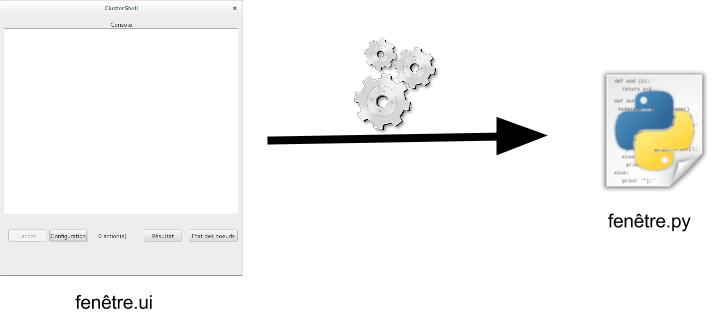
\includegraphics[scale=0.3]{conversion_ui_py.jpg}
\caption{Conversion ui - py}
\end{figure}

Pour convertir on utilise la commande suivante: \textbf{pyuic4 fenêtre.ui > fenêtre.py}

\subsubsection{Les signaux et les slots}
Pour de la programmation événementielle, on utilise deux moyens qui sont propres à Qt: les signaux et les slots. Chaque composant graphique (comme un bouton) possède des signaux et des slots qui vont permettre d'intéragir avec d'autres composants et fonctions(exemple: ouvrir une fenête via un bouton).\\
\linebreak
\textbf{Un signal:} Un signal est un message envoyé par une classe lors du déclenchement d'un événement comme le clic sur un bouton\\
\textbf{Les slots:} Les slots sont tout simplement des fonctions qui seront déclenchés par les signaux. Les fonctions peuvent être créés par nous même ou cela peut être des fonctions propres à une classe de Qt( exemple: la fonction \textbf{quit} de \textbf{QApplication} qui quitte le programme.\\
Voici un petit exemple pour mieux comprendre:\\
\begin{figure}[hbtp]
\centering
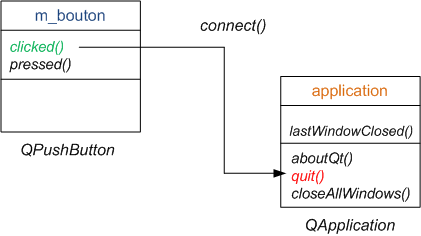
\includegraphics[scale=0.5]{exemple_signal_slot.png}
\caption{Les signaux et slots}
\end{figure}\\
Pour pouvoir assigner un slot à un signal on doit utilise la fonction \textbf{connect} que l'on définit dans la classe de notre fenêtre:
\begin{center}
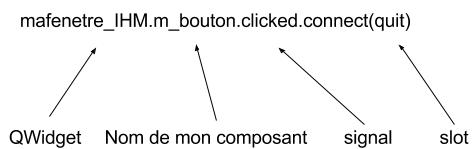
\includegraphics[scale=0.4]{signal_slot.jpg} 
\end{center}

\section{Sources}
\label{sec:section5}
\textbf{Nodeset:} \url{http://clustershell.readthedocs.io/en/latest/api/NodeSet.html}\\
\textbf{Task:} \url{http://clustershell.readthedocs.io/en/latest/api/Task.html}\\
\textbf{Qt GUI:} \url {http://doc.qt.io/qt-4.8/qtgui-module.html}\\
\url {https://pythonspot.com/en/pyqt4/}\\
\url {http://pyqt.sourceforge.net/Docs/PyQt4/qtgui.html}

\end{document}